\documentclass[]{cv-style}

\sethyphenation[variant=british]{english}{}

\begin{document}

\header{Stefan}{Kapferer}{Software Engineer}

%----------------------------------------------------------------------------------------
%	SIDEBAR SECTION  -- In the aside, each new line forces a line break
%----------------------------------------------------------------------------------------

\begin{aside}
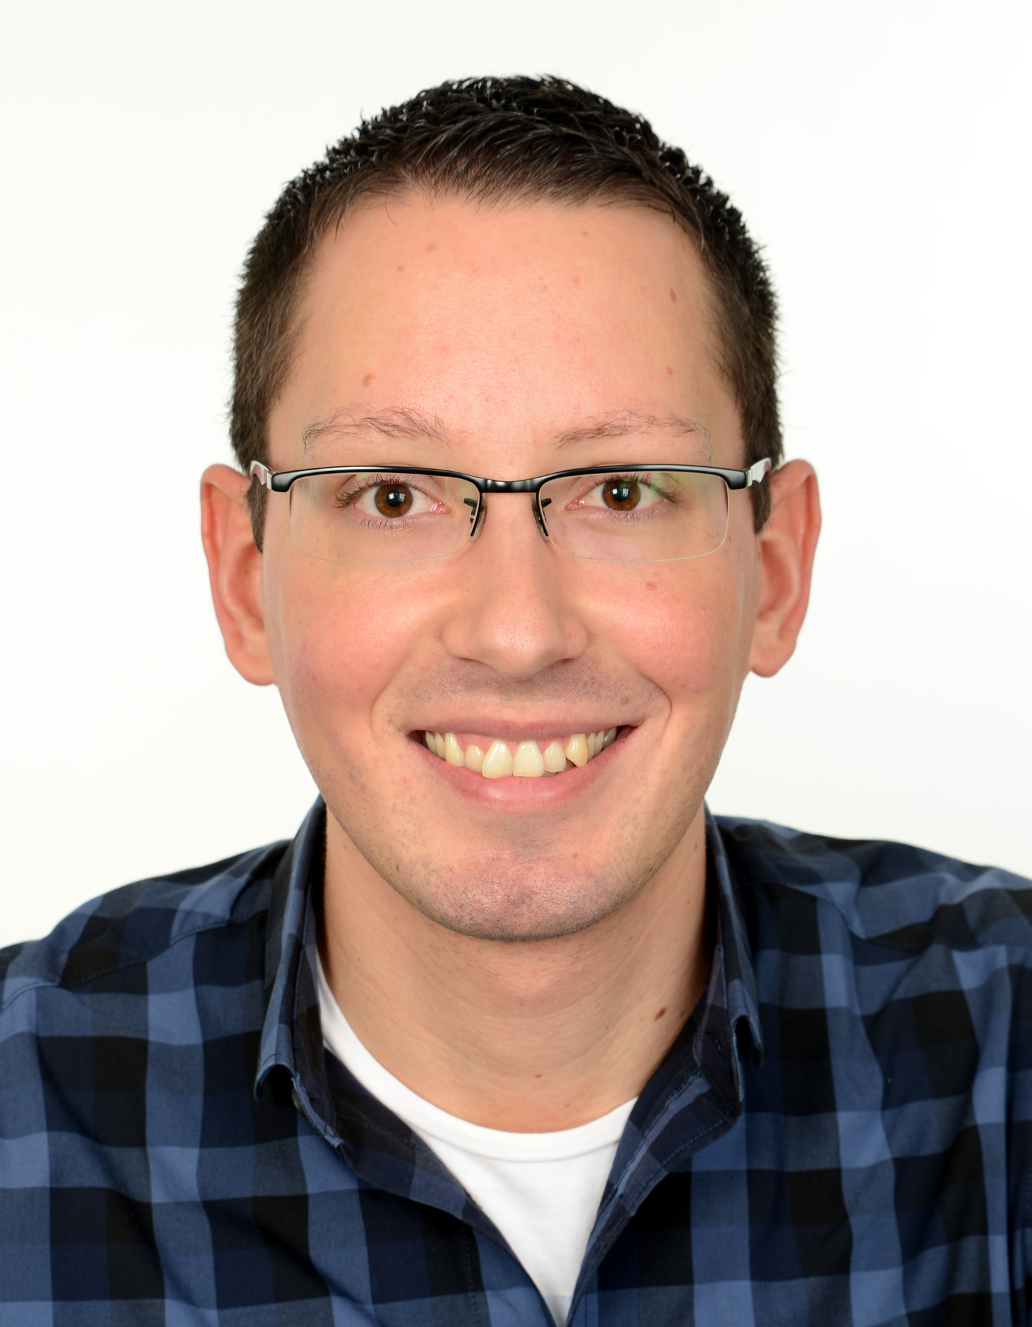
\includegraphics[width=3.5cm]{ska}
%
\section{contact}
Neue Jonastrasse 75
8640 Rapperswil SG
Switzerland
%~
%+41 78 898 31 80
~
stefan@kapferer.ch
%
\section{web \& github}
\href{https://stefan.kapferer.ch}{stefan.kapferer.ch}
\href{https://twitter.com/stefankapferer}{@stefankapferer}
\href{https://github.com/stefan-ka}{github.com/stefan-ka}
%
\section{languages}
german mother tongue
english fluency
%
\section{interests}
software engineering\smallskip
software architecture and design\smallskip
service-oriented architectures\smallskip
microservices\smallskip
domain-driven design\smallskip
object-oriented analysis and design\smallskip
concepts of object-oriented programming\smallskip
java\smallskip
%
\end{aside}

%----------------------------------------------------------------------------------------
%	WORK EXPERIENCE SECTION
%----------------------------------------------------------------------------------------

\section{experience}

\begin{entrylist}
%------------------------------------------------
\entry
  {2020--Now}
  {\href{https://ifs.hsr.ch}{Institute for Software (IFS)} at \href{https://www.hsr.ch}{HSR}}
  {Rapperswil}
  {\jobtitle{Software Engineer and Project Lead}
  \begin{itemize}
  	\item Software engineer and project lead in the \href{https://contextmapper.org/}{Context Mapper} open source project
  	\item Research projects around Domain-driven Design (DDD), service-oriented architectures / microservices, and service decomposition
  \end{itemize}}
%------------------------------------------------
\entry
  {05--09 2018}
  {\href{https://www.ergon.ch}{Ergon Informatik AG}}
  {Zurich}
  {\jobtitle{Internship in Software Engineering}
  \begin{itemize}
  	\item Implementation of business web application in the real estate industry
  	\item Implementation and maintenance of build- and testing platforms
  	\item Conducting customer training and a requirements engineering workshop
  \end{itemize}
  Used technologies and frameworks: HTML, CSS, JS, Freemarker, Java, Magnolia CMS, Gradle, Maven, Ansible}
%------------------------------------------------
\entry
  {2014--2017}
  {\href{https://www.adcubum.com}{Adcubum AG}}
  {St. Gallen}
  {\jobtitle{Software Engineer Professional (part-time: 60\%)}
  \begin{itemize}
    \item Design and implementation of tools to support developers \\(Eclipse plugins, command line tools, etc.)
    \item Development and realization of concepts concerning CI/CD
    \item Development, operation and maintenance of 'adcubum SYRIUS' build and it's continuous integration environment with Gradle and Jenkins
    \item Development, integration and operation of software documentation tools
    \item Classic software engineering tasks with Java and J2EE
    \item Documentation of architecture and design
    \item Supporting the migration from SVN to GIT
    \item Supporting developers regarding IDE (Eclipse), Build (Gradle), SCM (Git), Continuous Integration, etc.
  \end{itemize}}
%------------------------------------------------
\entry
  {2012--2013}
  {\href{https://www.adcubum.com}{Adcubum AG}}
  {St. Gallen}
  {\jobtitle{Software Engineer}\\
  Product development (adcubum SYRIUS):
  \begin{itemize}
    \item Development of new features and enhancements in the module \\'Bestandes-/Vertragsverwaltung'
    \item Creation of SQL scripts for database migration (Oracle DB)
    \item Architecture optimization for business processes within the module
    \item Supporting software quality assurance processes
  \end{itemize}
  Used systems and technologies: Java, JEE, Eclipse, SVN, Oracle SQL, XML, Linux}
%------------------------------------------------
\entry
  {2011--2012}
  {\href{https://www.swoffice.ch/}{swoffice ag}}
  {Teufen}
  {\jobtitle{Software Developer Java}
  \begin{itemize}
  	\item Product development (CRM solution)
  	\item Testing and operating solution (cloud-based solution)
  	\item Collaboration with customers in multiple projects
  \end{itemize}
  Technologies: Java, JavaFX, Spring Framework, Apache Lucene, PostgreSQL}
%------------------------------------------------
\end{entrylist}

\begin{entrylist}
\entry
  {2008--2011}
  {\href{https://www.clavisit.com/}{clavis IT ag}}
  {Herisau}
  {\jobtitle{Software Developer}
  \begin{itemize}
  	\item Development of solution concepts
  	\item Specification and design of solutions in direct collaboration with customers
  	\item Implementation of solutions based on the following technologies, frameworks and products: IBM Lotus Notes/Domino, Liferay Portal, Java/JEE (Tomcat and WebSphere Express), Web technologies (CSS, JS, HTML, XML), Webservices
  	\item Testing and documentation
  	\item Supporting customers with operating implemented solutions
  	\item Support and train apprentices
  \end{itemize}}
%------------------------------------------------
\entry
  {2004--2008}
  {\href{https://www.clavisit.com/}{clavis IT ag}}
  {Herisau}
  {\jobtitle{Apprenticeship in informatics (application development)}\\
  Software development using Java, Lotus Notes/Domino, and web technologies}
%------------------------------------------------
\end{entrylist}

%----------------------------------------------------------------------------------------
%	EDUCATION SECTION
%----------------------------------------------------------------------------------------

\section{education}

\begin{entrylist}
%------------------------------------------------
\entry
  {2018--2020}
  {M.Sc. {\normalfont in Engineering}}
  {\href{https://www.hsr.ch}{University of Applied Sciences of Eastern Switzerland (HSR FHO)}}
  {\jobtitle{Focusing on Information and Communication Technologies in the \\Software and Systems Master Research Unit}
  \\Conducted several research projects on the topics service decomposition, (micro-) service-oriented interfaces and architectures, and Domain-driven Design (DDD) aiming to strengthen personal knowledge in software architecture. The open source tool \href{https://contextmapper.org/}{Context Mapper} is a result of these projects.}
%------------------------------------------------
\entry
  {2017--2018}
  {Completed 21 credits towards a M.Sc. in Computer Science}
  {\href{https://www.ethz.ch}{ETH Zurich}}
  {Completed the following courses: Algorithms and Data Structures, Theoretical Computer Science, Linear Algebra}
%------------------------------------------------
\entry
  {2013--2017}
  {B.Sc. {\normalfont in Computer Science}}
  {\href{https://www.hsr.ch}{University of Applied Sciences of Eastern Switzerland (HSR FHO)}}
  {Developed a concept and prototypic implementation for an architectural refactoring of the data access security based on attribute-based access control (ABAC) in a standard software for the insurance sector.}
%------------------------------------------------
\entry
  {2009--2012}
  {Advanced Federal Diploma of Higher Education (HF) {\normalfont in Computer Science}}
  {\href{https://www.zbw.ch}{ZbW}}
  {Concept for a ``State of the art Java development environment with Continuous Integration (CI)'' and implementation in a case study project.}
%------------------------------------------------
\entry
  {2004--2008}
  {Apprenticeship {\normalfont in informatics (application development)}}
  {\href{https://www.clavisit.com}{clavis IT ag}}
  {\jobtitle{Federal Diploma of Vocational Education and Training (EFZ)}}
%------------------------------------------------
\end{entrylist}

%----------------------------------------------------------------------------------------
%	PAPERS & PUBLICATIONS SECTION
%----------------------------------------------------------------------------------------

\section{papers and publications}

\begin{entrylist}
%------------------------------------------------
\entry
{2020}
{\href{https://doi.org/10.5220/0008910502990306}{Domain-specific Language and Tools for Strategic Domain-driven Design, \\ Context Mapping and Bounded Context Modeling}}
{\href{http://www.modelsward.org/?y=2020}{MODELSWARD 2020}}
{In \textit{Proceedings of the 8th International Conference on Model-Driven Engineering and Software Development - MODELSWARD}, pages 299–306. INSTICC, SciTePress.}
%------------------------------------------------
\entry
{2020}
{\href{https://eprints.hsr.ch/821/}{A Modeling Framework for Strategic Domain-driven Design \\\ and Service Decomposition}}
{Master thesis at \href{https://www.hsr.ch}{HSR}}
{Proposing a modular architecture for a Strategic Domain-driven Design (DDD) modeling framework including a DSL, a reverse engineering framework, Architectural Refactorings (ARs), service decomposition analysis on the basis of coupling criteria, and multiple graphical generators. Have a look at the open source project \\ \href{https://contextmapper.org}{https://contextmapper.org} for more information.}
%------------------------------------------------
\entry
{2019}
{\href{https://eprints.hsr.ch/784/}{Service Decomposition as a Series of Architectural Refactorings}}
{Term project at \href{https://www.hsr.ch}{HSR}}
{Architectural Refactorings (ARs) derived from Decomposition Criteria (DCs) compiled from literature and own experience. Implemented as code refactorings for the \href{https://contextmapper.org/}{Context Mapper} tool.}
\end{entrylist}

\begin{entrylist}
\entry
{2019}
{\href{https://github.com/stefan-ka/papers-and-publications/raw/master/empirical-research-in-software-engineering/FS19_SKapferer_Empirical-Research-in-Software-Engineering-Paper.pdf}{Empirical Research in Software Engineering}}
{Seminar paper at \href{https://www.hsr.ch}{HSR}}
{Scientific research strategies applied to software engineering.}
%------------------------------------------------
\entry
{2018}
{\href{https://eprints.hsr.ch/722/}{A Domain-specific Language for Service Decomposition}}
{Term project at \href{https://www.hsr.ch}{HSR}}
{A formal approach to strategic Domain-driven Design (DDD) and service decomposition implemented in the \href{https://contextmapper.org/}{Context Mapper open source tool}.}
%------------------------------------------------
\entry
{2018}
{\href{https://stefan.kapferer.ch/model-transformations-for-dsl-processing}{Model Transformations for DSL Processing}}
{Seminar paper at \href{https://www.hsr.ch}{HSR}}
{Proof of concept for the implementation of refactorings for Domain-specific Languages (DSLs) on the basis of the Henshin tool and algebraic graph transformations.}
%------------------------------------------------
\entry
{2017}
{''\href{https://eprints.hsr.ch/602/}{Attributbasierte Autorisierung in einer Branchenlösung\\für das Versicherungswesen}''}
{Bachelor thesis at \href{https://www.hsr.ch}{HSR}}
{Concept and prototypic implementation for attribute-based access control in a (micro-)service-oriented architecture.}
%------------------------------------------------
\entry
{2016}
{''\href{https://eprints.hsr.ch/564/}{Architectural Refactoring der Data Access Security}''}
{Semester thesis at \href{https://www.hsr.ch}{HSR}}
{Extracting the data access security of a monolithic application into a separate Bounded Context (DDD) or microservice.}
%------------------------------------------------
\end{entrylist}

%----------------------------------------------------------------------------------------
%	TALKS SECTION
%----------------------------------------------------------------------------------------

\section{talks}

\begin{entrylist}
%------------------------------------------------
\entry
{2019}
{\href{https://www.jug.ch/html/events/2019/context_mapper.html}{Context Mapper: DSL and Tools for Domain-Driven Service Design}}
{\href{https://www.jug.ch/}{Java User Group CH}}
{Bounded context modeling and microservice decomposition}
%------------------------------------------------
\end{entrylist}
%----------------------------------------------------------------------------------------

\end{document}
